%!TEX root = ../master.tex
\chapter{Background Research}\label{ch:bgres}
\todo{introduction to this chapter is needed. It needs an explanation to why this chapter is relevant}
The background research in this chapter is based on acquiring answers to the initial problem statement and the two research questions. The research includes studies of state of the art artefacts, previous work and which methods they used. 
\section{Previous scientific work}
In this section, other attempts to digitally augment board games will be discussed.

Andersen et al. \citep{andersen_designing_2004} created "BattleBoard3D", a board game utilising physical and digital components. For their physical components they used flat squares with patterns that through Augmented Reality (AR) technologies will be recognised through a camera and/or Virtual Reality goggles. Their research was made to illustrate "design issues for AR board games".

Peitz et al. \citep{peitzWizards2006} created "Wizard's Apprentice", a computer-augmented board game. The game includes two roles: wizard and apprentice. All players but one play as apprentices guided by the wizard who acts as a negotiator and motivator. The software is written in Java and has several play modes. The game uses Radio-Frequency Identification (RFID) hardware to detect at which physical point the players are in the game. It sends this information through antennas to a laptop close by. The laptop projects this information to a screen that displays relevant information on each player's turn. The game board can be seen in Figure \ref{fig:peitz}.

\begin{figure}[!h]
\centering	
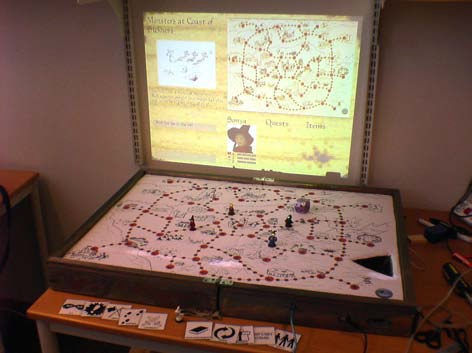
\includegraphics[width=0.5\textwidth]{peitz}
\caption{The Wizard's apprentice game board setup from \citep{peitzWizards2006}}
\label{fig:peitz}
\end{figure}

\section{Commercial competition}
Apart from previous scientific work, commercial board games have been released, existing on a spectrum ranging from completely digital to completely analogue. As our product will exist somewhere on the spectrum, these commercial solutions can be considered state of the art for this project.

On the digital end, the online collectible card game Hearthstone (for Windows, OS X, Android and iOS), though completely virtual, has an interface which resembles a physical game board with cards and information on it. The user plays the game by dragging the cards onto the board from their 'hand' by way of using the cursor (when playing on a desktop computer), or by swiping with a finger (when playing on a smartphone or a tablet). The cards placed on the board can then be dragged to the cards they need to attack, etc. This swiping mechanism gives the game a tangible sense, making it resemble an analogue card game, even though no physical cards are involved.

\todo{do we also need games originally designed as a board game and late made digital?}




\todo{This section will describe some of the commercial solutions. We will describe how they exist on a spectrum which ranges from completely digital to completely analogue board games:

 - Hearthstone/Marioparty
 
 - Trivial pursuit digital udgave / wordfeud
 
 - Xcom game / Golem Arcana
 
 - Munchkin level counter
 
 - Monopoly m kreditkort/jeopardy m buzzer
 
 - 100percent analogue board games}

\section{Methods for evaluating and measuring key success criteria}
Andersen et al. \citep{andersen_designing_2004} evaluated their product on a group of 13 year old children. The goals were to "reveal issues concerning the game design in general, design of the physical pieces, the use of goggles versus screen display, and future evolvement." The children found the 3D projection of the characters through the goggles fascinating, although some fumbling with the game pieces occurred due to the nature of the goggles and placement of the webcam. This occurred less when they looked at the 3D figures on the screen, but this brought along the problem of shifting focus away from the board game.
Finally, the children found the small set of animations uninteresting after a while and suggested a higher number of animations were needed to keep interest.

Peitz et al. \citep{peitzWizards2006} performed an initial evaluation on 3 children aged 8-9 and a male adult player (37). The evaluation was based upon a template that evaluates the social adaptability of game divided into: "(...)spatial, temporal, social, and playability." The participants were observed for two hours and were thematically interviewed afterwards. The participants reported overall enjoyment and increased togetherness in the game, but the pacing of the game felt unfamiliar. The participants seemed to particularly react positively to the sound design. 

\begin{figure}[!h]
\centering	
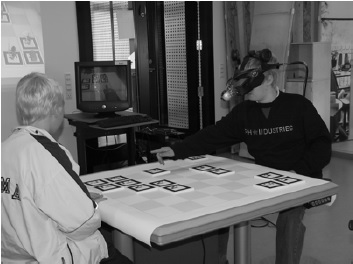
\includegraphics[width=0.5\textwidth]{andersen}
\caption{BattleBoard3D setup from Andersen et al.  \citep{andersen_designing_2004}}
\label{fig:andersen}
\end{figure}

\section{Competitive analysis}
As shown in \citep{andersen_designing_2004}, a solution to enhance a board game can be done through AR aided by either a screen or Virtual Reality (VR) goggles. Andersen et al. mention some drawbacks to both of their technologies. In the case of AR with a screen they note that while the screen gives the participants the ability to look their opponent in the eye, they are distracted by having to look away from the board game space, to look at the screen displaying the figures. Regarding the VR, they note that participants liked the ability to pick up a game piece and explore all sides of the 3D model through the goggles. The problem, as can be seen in Figure \ref{fig:andersen}, could be that the goggles take away from the non-verbal communication that board games tend to foster.

In \citep{peitzWizards2006} Peitz et al. built a board together with RFID antennas and other hardware to detect certain points of the the players' progression. They note some positive things, as aforementioned, namely the increased feeling of togetherness and overall enjoyment. They follow a recipe most traditional board games follow: a tile progression. They simulate this with the dots throughout the map, which the "tokens" press down on and activate. They also note the relationship between wizard and apprentices works well, but note an interesting development in the dynamics when one of the children effectively demotes the adult, who has the role as wizard, and temporarily acts as a new wizard. They did not account for this, but mention it is within their design goals.